\documentclass{article}
\usepackage{amsmath}
\usepackage{amssymb}
\usepackage{graphicx}
\usepackage{hyperref}
\usepackage[version=4]{mhchem}

\title{Example 9}
\date{}

\begin{document}
\maketitle

\(\triangle A B C\) is a right triangle with \(\angle A C B=90^{\circ}\). Points \(D\) and \(E\) are the midpoints on sides \(A B\) and \(A C\), respectively. Extend \(B C\) to \(F\) such that \(C F=\frac{1}{2} B C\). Connect \(C F\). Show that \(\angle B=\angle F\).\\
\centering
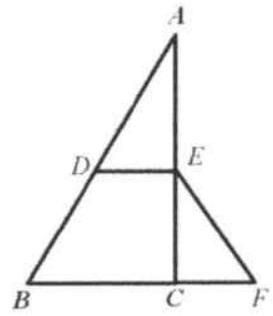
\includegraphics[width=\textwidth]{images/problem_image_1.jpg}


Solution:
Draw \(D C\), the median of triangle \(A B C\). Since \(D C\) is the median, by Theorem 1.3, \(D C=B D\).\\
Since \(A D=\frac{1}{2} F C, A D=D N\). So that \(\angle B=\angle D C B\).\\
Since points \(D\) and \(E\) are the midpoints on sides \(A B\) and \(A C\), \(D E=\frac{1}{2} B C=C F\) and \(D E / / B C\). Thus \(D E F C\) is a\\
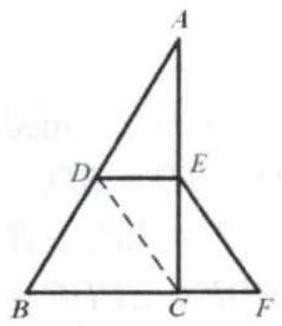
\includegraphics[width=\textwidth]{images/reasoning_image_1.jpg} parallelogram. So \(D C / / E F\) and \(\angle D C B=\angle F\).\\
Since \(\angle B=\angle D C B, \angle B=\angle F\).


\end{document}
